En esta sección se presentan los resultados obtenidos a partir de las distintas ejecuciones realizadas. \\

\subsection{Resultados objetivo específico 1: MapReduce vs Hive (\textit{external tables}) vs Pig}

A continuación se ilustran los distintos tiempos de ejecución obtenidos a partir de las pruebas realizadas con el programa \textit{MaxTemperature} en las versiones MapReduce-Java, Pig, y Hive para el total y el 10\% de los datos del NCDC. La figura \ref{07_01_01} compara los tiempos de ejecución del programa \textit{MaxTemperature} en la versión MapReduce-Java con el total y el 10\% de los datos. La figura \ref{07_01_02} compara los tiempos de ejecución del programa \textit{MaxTemperature} en la versión Pig con el total y el 10\% de los datos. La figura \ref{07_01_03} compara los tiempos de ejecución del programa \textit{MaxTemperature} en versión Hive en su forma nativa (Hive server) y desde Hue (\textit{managed tables}) con el total de los datos. La figura \ref{07_01_04} compara los tiempos de ejecución del programa \textit{MaxTemperature} en las versiones MapReduce-Java, Hive (\textit{external tables}), y Pig con el total de los datos.

\begin{figure}[H]
  \centering
      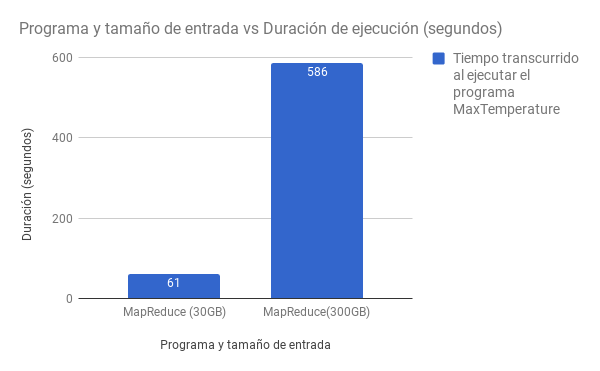
\includegraphics[width=\textwidth, height=3.0in]{fig/07/01_01}
  \caption{Comparación de MapReduce-Java con el total y el 10\% de los datos.}
  \label{07_01_01}
\end{figure}

\begin{figure}[H]
  \centering
      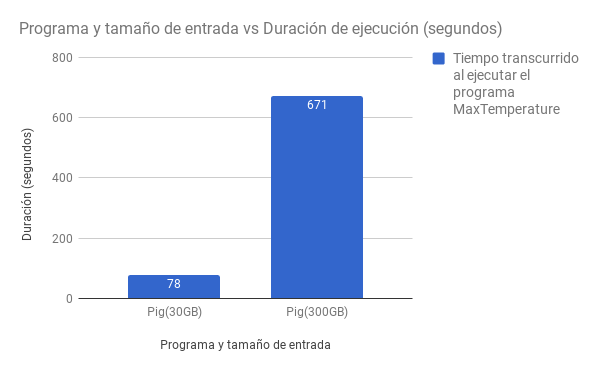
\includegraphics[width=\textwidth, height=3.0in]{fig/07/01_02}
  \caption{Comparación de Pig con el total y el 10\% de los datos.}
  \label{07_01_02}
\end{figure}

\begin{figure}[H]
  \centering
      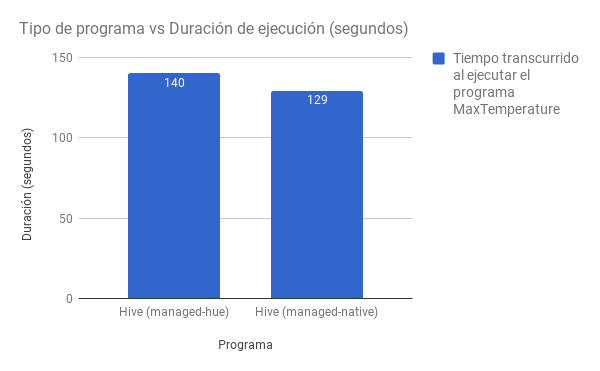
\includegraphics[width=\textwidth, height=3.0in]{fig/07/01_03}
  \caption{Comparación de ejecución en Hive de forma nativa y desde Hue con el total de los datos.}
  \label{07_01_03}
\end{figure}

\begin{figure}[H]
  \centering
      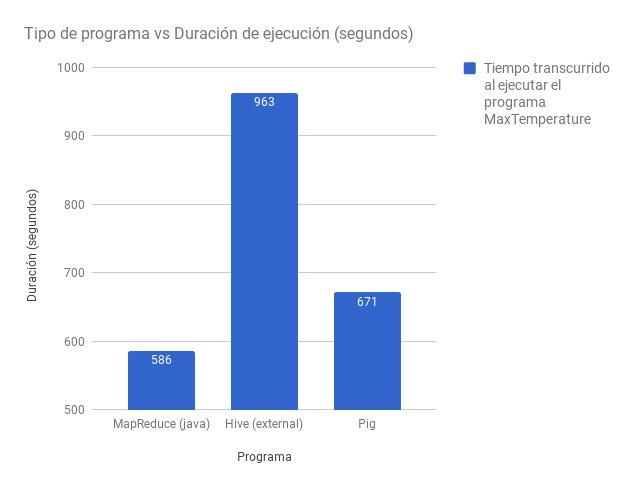
\includegraphics[width=\textwidth, height=3.5in]{fig/07/01_04}
  \caption{Comparación de ejecución del programa \textit{MaxTemperature} desde MapReduce, Hive (\textit{external table}), y Pig con el total de los datos.}
  \label{07_01_04}
\end{figure}

\subsection{Resultados objetivo específico 2: Escalabilidad en Pig}

A continuación se ilustran los distintos tiempos de ejecución obtenidos a partir de las pruebas realizadas con el programa \textit{AverageTemperatureCount} para medir la escabilidad de Pig. Para esto, dos distintos enfoques fueron usados: el primero consistía en deshabilitar, mediante la interfaz gráfica de YARN, NodeManagers y trabajar con el total de DataNodes (10 en nuestro caso); el segundo consistía en agregar nuevos nodos al cluster y ejecutar los scripts cada vez que esto sucedía, lo que significaba que las instancias de NodeManagers activas eran igual a los nodos en los que se encontraban replicados los datos. La figura \ref{07_02_01} muestra los resultados del primer enfoque, mientras que la figura \ref{07_02_02} muestra los del segundo.

\begin{figure}[H]
  \centering
      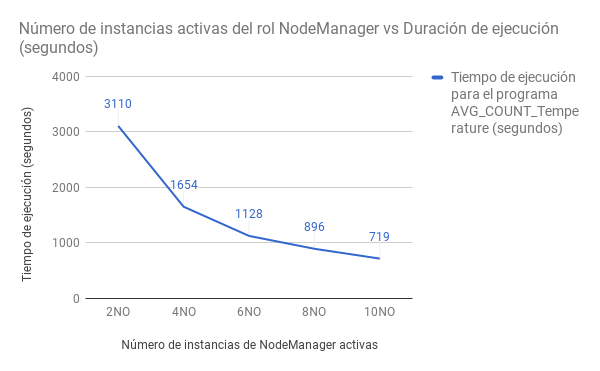
\includegraphics[width=\textwidth, height=3.0in]{fig/07/02_01}
  \caption{Escalabilidad de Pig en términos del procesamiento de datos (Pig/YARN).}
  \label{07_02_01}
\end{figure}

\begin{figure}[H]
  \centering
      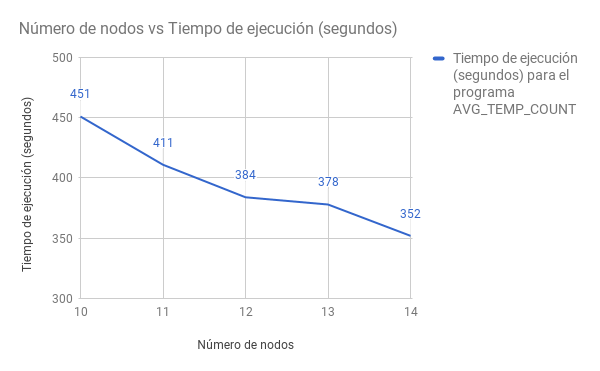
\includegraphics[width=\textwidth, height=3.0in]{fig/07/02_02}
  \caption{Escalabilidad de Pig (Pig/HDFS/YARN).}
  \label{07_02_02}
\end{figure}

Para analizar los resultados evidenciados en las gráficas anteriores, se transformaron los tiempos de ejecución (eje vertical) a una escala logarítmica y se uso la función \textit{lm} del lenguaje de programación R para comprobar si en efecto la escalabilidad era logarítmica. A continuación se presentan los resultados arrojados. \\

\subsubsection{Análisis de la escalabilidad de Pig siguiendo el enfoque 1}

\begin{itemize}

\item \textbf{Función de transformación:} $log(y)$
\item \textbf{p-value:} 0.002416

\end{itemize}

\subsubsection{Análisis de la escalabilidad de Pig siguiendo el enfoque 2}

\begin{itemize}

\item \textbf{Función de transformación:} $log(y)$
\item \textbf{p-value:} 0.004018

\end{itemize}

\subsection{Resultados objetivo específico 3: Extensibilidad de Pig con HCatalog:}

A continuación se ilustran los distintos tiempos de ejecución y tamaños de lectura de datos desde HDFS obtenidos a partir de las pruebas realizadas con el programa \textit{AverageTemperature} para medir la extensibilidad de Pig con HCatalog y su influencia en los tiempos de ejecución. La figura \ref{07_03_01} muestra la comparación en los tiempos de ejecución para el programa \textit{AverageTemperature-1950} de Pig con HCatalog (con una tabla no particionada), Pig con HCatalog (con una tabla particionada), y de Pig sin HCatalog. La figura \ref{07_03_02} muestra la comparación de la lectura de datos desde HDFS para el programa \textit{AverageTemperature-1950} de Pig con HCatalog (con una tabla no particionada), Pig con HCatalog (con una tabla particionada), y de Pig sin HCatalog. La figura \ref{07_03_03} muestra la comparación en los tiempos de ejecución para el programa \textit{AverageTemperature-1910} de Pig con HCatalog (con una tabla no particionada), Pig con HCatalog (con una tabla particionada), y de Pig sin HCatalog. La figura \ref{07_03_04} muestra la comparación de la lectura de datos desde HDFS para el programa \textit{AverageTemperature-1910} de Pig con HCatalog (con una tabla no particionada), Pig con HCatalog (con una tabla particionada), y de Pig sin HCatalog.


\begin{figure}[H]
  \centering
      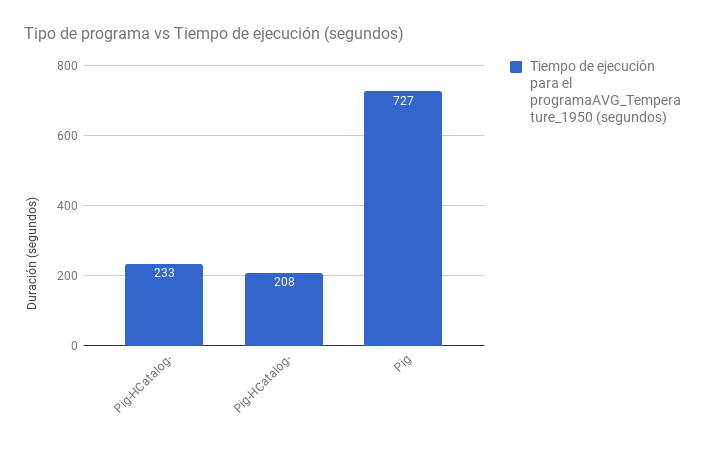
\includegraphics[width=\textwidth, height=4.0in]{fig/07/03_01}
  \caption{Tiempos de ejecución obtenidos para el programa \textit{AverageTemperature-1950}.}
  \label{07_03_01}
\end{figure}

\begin{figure}[H]
  \centering
      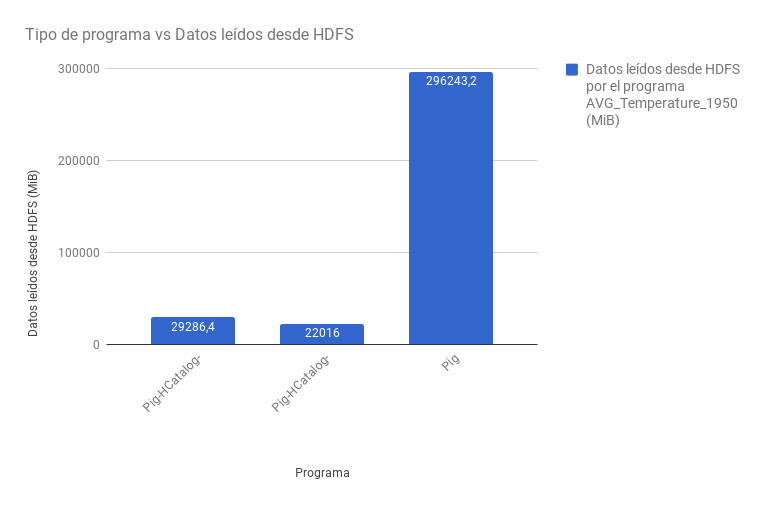
\includegraphics[width=\textwidth, height=4.0in]{fig/07/03_02}
  \caption{Lectura de datos desde HDFS para el programa \textit{AverageTemperature-1950}.}
  \label{07_03_02}
\end{figure}

\begin{figure}[H]
  \centering
      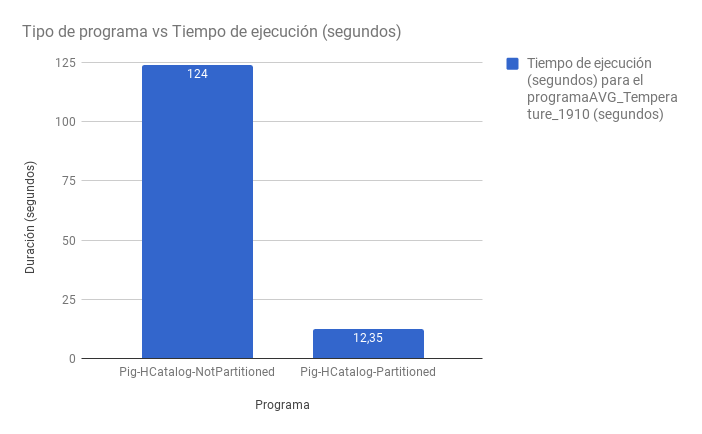
\includegraphics[width=\textwidth, height=4.0in]{fig/07/03_03}
  \caption{Tiempos de ejecución obtenidos para el programa \textit{AverageTemperature-1910}.}
  \label{07_03_03}
\end{figure}

\begin{figure}[H]
  \centering
      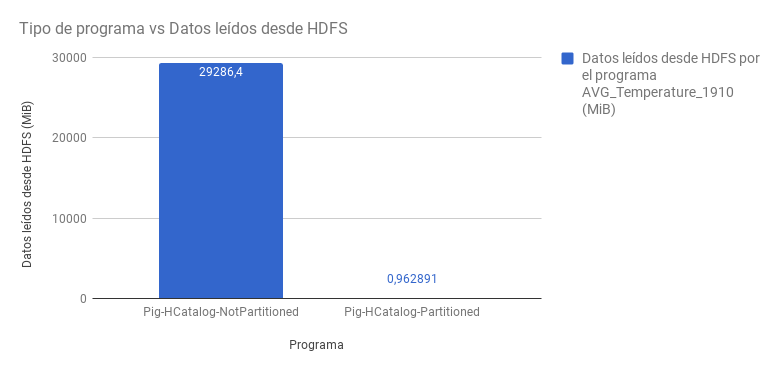
\includegraphics[width=\textwidth, height=4.0in]{fig/07/03_04}
  \caption{Lectura de datos desde HDFS para el programa \textit{AverageTemperature-1910}.}
  \label{07_03_04}
\end{figure}

\subsection{Resultados objetivo específico 4: Reusabilidad y mantebilidad en Oozie}

La reusabilidad y mantenibilidad de los \textit{workflows} de Oozie se pudo comprobar al lograr intercambiar fácilmente el primer \textit{stage} del mismo.  La figura \ref{07_04_01} ilustra los tiempos de ejecución obtenidos a partir de las pruebas realizadas con las definiciones del \textit{workflow} en sus versiones: Pig-Pig y Hive-Pig.

\begin{figure}[H]
  \centering
      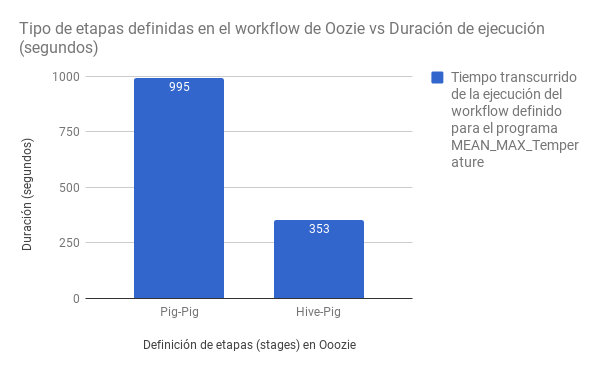
\includegraphics[width=\textwidth, height=4.0in]{fig/07/04_01}
  \caption{Comparación del \textit{workflow} de Oozie con la combinación Pig-Pig y Hive-Pig.}
  \label{07_04_01}
\end{figure}